\subsection{State of the Art}
\label{sec:intro:stateoftheart}

HOPR has been built on top of, or as a reaction to, various technologies and research projects which try to meet some or all of the design ethos and security goals outlined above. These technologies and research projects can be broadly divided into three groups: (1) \lcnameref{sec:intro:stateoftheart:privacyprotocols} which attempt to hide user information; (2) \lcnameref{sec:intro:stateoftheart:l2protocols} which allow systems to perform micro-payments via the Ethereum blockchain, as well as (3) \lcnameref{sec:intro:stateoftheart:p2pnetworks} which allow nodes to interact with each other directly without requiring a central coordinator. The following sections present the state of the art for each of these groups.

\subsubsection{Anonymous Communication Protocols}
\label{sec:intro:stateoftheart:privacyprotocols}

\paragraph{Virtual Private Networks}(\textit{VPNs}) are point-to-point overlay networks used to create secure connections over an otherwise untrusted network, such as the internet \cite{venkateswaran_2001}. Clients receive a public IP address from the VPN endpoint, which is then used for all outgoing communication. Since this public IP address can be almost anywhere in the world, VPNs are often used to bypass censorship \cite{hobbs_roberts_2018} and geolocalization blocks. However, VPNs provide dubious privacy, since clients must trust the VPN endpoint. The endpoint provider has full access to users' connection and communication metadata, since they control all communication going through it. In addition, VPN endpoints are often a single point of failure, since they are provided as centralized services. Both factors are major weaknesses when considering VPNs for privacy-preserving communication.

These privacy concerns have motivated the creation of a new model for VPNs, \textbf{Decentralized Virtual Private Networks} (\textit{dVPN}s). dVPNs leverage blockchain technology to remove reliance on a central authority. Users act as bandwidth providers, allowing other users to access internet services via their node, in exchange for rewards.

Examples of dVPN projects include Orchid \cite{orchid}, Sentinel \cite{sentinel}, and Mysterium \cite{mysterium}. However, these projects still lack privacy, performance, and reliability guarantees, since bandwidth providers can potentially inspect, log, and share any of their traffic. This harms honest bandwidth providers as well as users: since bandwidth providers can theoretically monitor traffic, nodes whose bandwidth are used to enable illicit activity can potentially be held liable for those activities by government authorities. Indeed, there have been incidents where unaware dVPN users have been (ab)used as exit nodes through which DDoS attacks
were performed.

A research project called VPN$^0$ \cite{vpn0} aims to provide better privacy guarantees. VPN$^0$ leverages zero-knowledge proofs to hide traffic content to relay nodes with traffic accounting and traffic blaming capabilities as a way to combat the weaknesses of other dVPN solutions.

\paragraph{Onion Routing} is another approach to network privacy, implemented by projects such as Tor \cite{tor}. Tor encapsulates messages in layers of encryption and transmits them through a series of network nodes called \textit{onion routers}. However, Tor is susceptible to end-to-end correlation attacks from adversaries who can eavesdrop on the communication channels. These attacks reveal a wide range of information, including the identity of the communicating peers.

The Invisible Internet Project (\textit{I2P}) is an implementation of onion routing with notably different characteristics than Tor \cite{i2p}:

\begin{itemize}

  \item \textbf{Packet switched instead of circuit switched}
        Tor allocates connection to long-lived circuits; this allocation does not change until either the connection or the circuit closes. In contrast, routers in I2P maintain multiple tunnels per destination. This significantly increases scalability and failure resistance since packets are used in parallel.

  \item \textbf{Unidirectional tunnels}
        Employing unidirectional rather than bidirectional tunnels makes deanonymization harder, because tunnel participants see half as much data and need two sets of peers to be profiled.

  \item \textbf{Peer profiles instead of directory authorities}
        I2P’s network information is stored in a DHT (information in the DHT is inherently untrusted) while Tor’s relay network is managed by a set of nine Directory Authorities.
\end{itemize}

Despite these improvements, I2P is vulnerable to eclipse attacks since no I2P router has a full view of the global network (similar to other peer-to-peer networks). Like Tor, I2P only provides protection against local adversaries, making it vulnerable to timing, intersection, and traffic analysis attacks. I2P has also been shown to be vulnerable to Sybil and predecessor attacks, in spite of various countermeasures implemented to thwart these.

\paragraph{Mixnets} are overlay networks of so-called \textit{mix nodes} which route packets anonymously, similarly to Tor \cite{mixnets}. Mixnets originally used a cascade topology where each node would receive a batch of encrypted messages, decrypt them, randomly permute packets, and transfer them in parallel. Cascade topology makes it easy to prove the anonymity properties of a given mixnet design for a particular mix. However, it does not scale well with respect to increasing mixnet traffic and is susceptible to traffic attacks. Since then, research has evolved to provide solutions with low latency while still providing high anonymity by using a method called \textit{cover traffic}. Cover traffic is designed to hide communication packets among random noise. An external adversary able to observe the packet flow should not be able to distinguish communication packets from these cover traffic packets, increasing privacy.

The application of cover traffic provides metadata protection from global network adversaries, a considerable improvement on projects such as Tor and I2P. However, because mixnets add extra latency to network traffic, they are better suited to applications that are not as sensitive to increased latency, such as messaging or email applications. For applications such as real-time video streaming, Tor may be more suitable, provided the user feels the latency improvements outweigh the increased privacy risks.

Loopix \cite{loopix} is another research project which uses cover traffic to resist traffic analysis while still achieving low latency. To achieve this, Loopix employs a mixing strategy called \textit{Poisson mix}. Poisson mix nodes independently delay packets, making packets unlinkable via timing analysis.

\subsubsection{Layer-2 Scalability Protocols}
\label{sec:intro:stateoftheart:l2protocols}

Blockchain technology (mostly public blockchains like Bitcoin and Ethereum) suffers from a major scalability issue: every node in the network needs to process every transaction, validate them, and store a copy of the entire chain state. Thus the number of transactions cannot exceed that of a single node. For Ethereum, this is currently around 30 transactions per second.

Multiple solutions have been proposed to resolve the scalability issue, including sharding and off-chain computation. Both approaches intend to create a second layer of computation to reduce the load on the blockchain mainnet.

Off-chain solutions such as Plasma \cite{plasma}, Truebit \cite{truebit}, and state channels process transactions outside the blockchain while still guaranteeing a sufficient level of security and finality. State channels are better known as ``payment channels". In models like the Lightning Network \cite{lightningnetwork}, a payment channel is opened between two parties by committing a funding transaction. Those parties may then make any number of signed transactions that update the channel's funds without broadcasting those to the blockchain. The channel is eventually closed by broadcasting the final version of the settlement transaction. The channel balance is updated by creating a new set of commitment transactions, followed by trade revocation keys which render the previous set of commitment transactions unusable. Both parties always have the option to ``cash out" by submitting the latest commitment transaction to the blockchain. If one party tries to cheat by submitting an outdated commitment transaction, the other party can use the corresponding revocation key to take all the funds in the channel.

As soon as closure is initiated, the channel can no longer be used to route payments. There are different channel closure transactions depending on whether both parties agree on closing the channel. If both agree, they provide a digital signature that authorizes this cooperative settlement transaction. In the case where they disagree or only one party is online, a unilateral closure is initiated without the cooperation of the other party. This is done by broadcasting a ``commitment transaction". Both parties will receive their portion of the money in the channel, but the party that initiates the closure must wait for a certain delay to receive their money. This delay time is negotiated by the nodes before the channel is opened, for the protection of both parties.

The Raiden network \cite{raiden} is a layer-2 payment solution for the Ethereum blockchain. The project employs the same technological innovations pioneered by the Bitcoin Lightning Network by facilitating transactions off-chain, but provides support for all ERC-20 compliant tokens. Raiden differs in operation from its main chain because it does not require global consensus. However, to preserve the integrity of transactions, Raiden powers token transfers using digital signatures and hash-locks. Known as \textbf{balance proofs}, this type of token exchange uses payment channels. Raiden also introduces ``mediated transfers", which allow nodes to send payments to another node without opening a direct channel to it. These payment channels are updated with absolute amounts, whereas HOPR employs relative amounts (more details in Section \ref{sec:tickets}).

\begin{comment}
We present in the following a comparison table (from the Loopix paper) between different anonymous communication systems.

\begin{figure}[H]
  \centering
  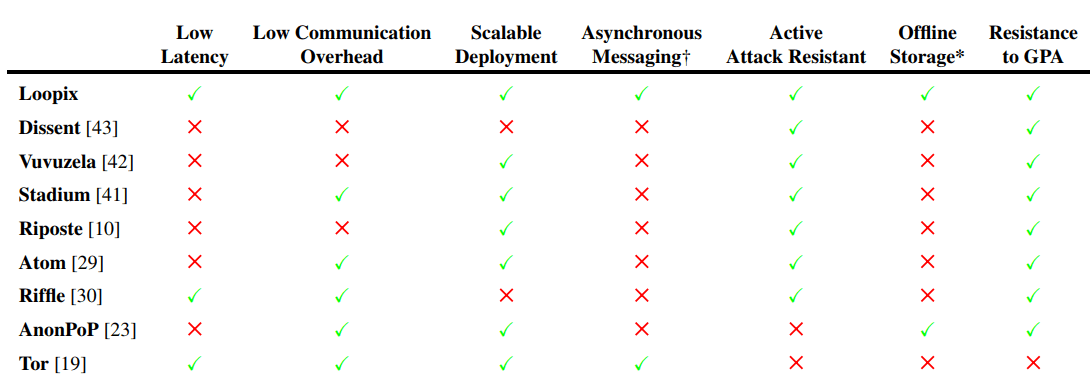
\includegraphics[width=11cm,height=11cm,keepaspectratio]{../yellowpaper/images/state-of-the-art.png}
  \caption{Comparison between anonymous communication systems}
  \label{fig:Comparison between anonymous communication systems}
\end{figure}
\end{comment}

\subsubsection{P2P Networks}
\label{sec:intro:stateoftheart:p2pnetworks}

% DHT 

% NAT Traversal